\section{Data preprocessing}
\label{section:Data:Preprocessing}
The way our data pipeline was constructued made it self documenting,
which means it prints out all the processing steps and saves them as the
experiment is conducted. This section will briefly cover how the data was processed
before each type of experiments.
The different model structures required some differences in processing steps.

\subsection{Common processing steps for all models}

\begin{table}[h]
  \centering
  \caption{Base data processing steps}
  \label{table:base_data_processing_steps}
  \begin{tabular}{ll}
    \toprule
    Step       & Description                                                   \\
    \midrule
    \textbf{1} & load market insight data and categories and merge them        \\
    \textbf{2} & convert date columns to date\_time format                     \\
    \textbf{3} & sum up clicks to category level [groupBy(date, cat\_id)]      \\
    \textbf{4} & rename column 'title' to 'cat\_name'                          \\
    \textbf{5} & combine feature 'hits' and 'clicks' to new feature 'interest' \\
    \textbf{6} & drop columns 'hits' and 'clicks'                              \\
    \textbf{7} & filter out data from early 2018-12-01                         \\
    \textbf{8} & drop uninteresting colums                                     \\
    \bottomrule
  \end{tabular}
\end{table}

\begin{table}[h]
  \centering
  \caption{LSTM data processing steps}
  \label{table:lstm_data_processing_steps}
  \begin{tabular}{ll}
    \toprule
    Step       & Description                                                                  \\
    \textbf{1} & Convert input dataset to generator object                                    \\
    \textbf{2} & filter out category 12322                                                    \\
    \textbf{3} & choose columns 'interest' and 'date'                                         \\
    \textbf{4} & fill in dates with zero values                                               \\
    \textbf{5} & convert to np.array                                                          \\
    \textbf{6} & scale data between 0.1 and 1                                                 \\
    \textbf{7} & generate x y pairs with sliding window with input size 10, and output size 7 \\
    \textbf{8} & generate training and validation data with training size 7                   \\
    \bottomrule
  \end{tabular}
\end{table}
\begin{table}[h]
  \centering
  \caption{LSTM data processing steps}
  \label{table:arima_data_processing_steps}
  \begin{tabular}{ll}
    \toprule
    Step       & Description                                                     \\
    \textbf{1} & Convert input dataset to generator object                       \\
    \textbf{2} & filter out category 2)                                          \\
    \textbf{3} & choose columns 'interest' and 'date'                            \\
    \textbf{4} & fill in dates with zero values                                  \\
    \textbf{5} & Scaling data?: False                                            \\
    \textbf{6} & split up into training set and test set of forecast window size \\
    \bottomrule
  \end{tabular}
\end{table}

TODO[Add Arima data preprocessing steps]
%\textbf{%} &Combine feature click and hit \\
%\textbf{%} &Filter out data from 2018 \\
%\textbf{%} &Sliding window of input output pairs \\
%\textbf{%} &Min max scaling \\
%\textbf{%} &Train val, test split \\

\subsubsection{Moving Window Approach}
We are using the same approach  as in \cite{Bandara2019} %Sales Demband FOrecast in E-commerce
and \cite{Hewamalage2021}% Current state and future predictions
\begin{figure}[h!]
  \centering
  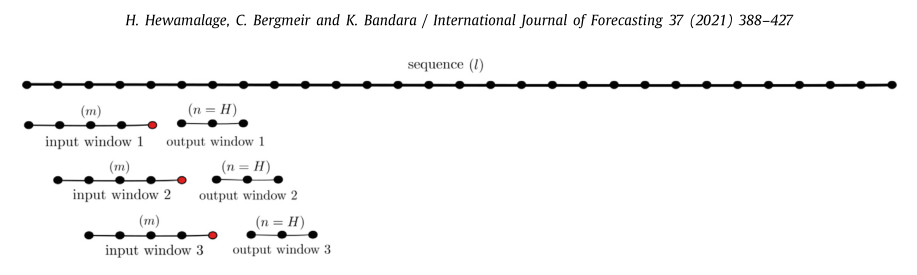
\includegraphics[width=\textwidth]{./figs/illustrations/moving_window_illustration.png}
  \hfill
  \caption{Moving window scheme \citep{Hewamalage2021}}
  \label{fig:dataset:moving_window_scheme}
\end{figure}